\chapter{RESULTS}
\label{chp:results}

In addition to employing grid search and built-in cross-validation to optimize the classifiers described in Chapter \ref{chp:methods}, the impact of two methods to rescale the features was evaluated: normalization and standardization. Furthermore, the influence of \gls{pca} by considering 98\% of the explained variance was also investigated, resulting in approximately 50\% reduction in the number of features. All analysis and results henceforth were evaluated in Excel, with examples using the ESC-10 dataset depicted in Figures \ref{fig:results_ESC-10_classification_results_overview} and \ref{fig:results_ESC-10_classification_results_fold_overview}. The results were compiled in the subsequent sections only as tables.

\begin{figure}[htbp]
    \centering
        \caption{Overview of the results of the classifiers during the training / classification flow — Example with the ESC-10 dataset.}
        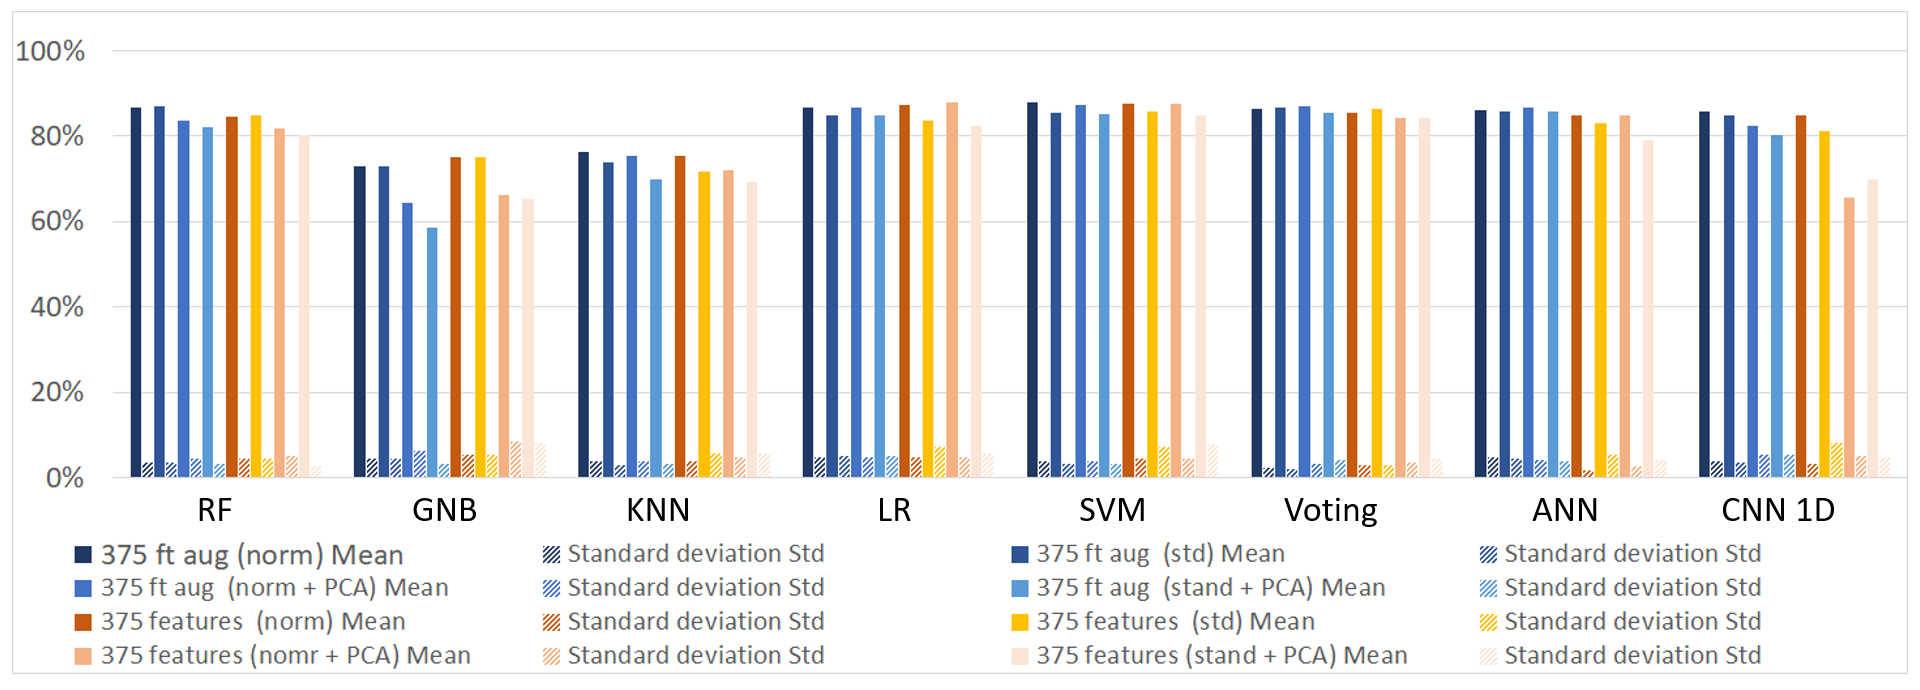
\includegraphics[width=1\textwidth]{resources/images/060-results/Results_classification_flow_ESC-10_2.png}
        \smallcaption{Source: Author}
        \label{fig:results_ESC-10_classification_results_overview}
\end{figure}

\begin{figure}[htbp]
    \centering
        \caption{Comparison of the best option for the classifiers results per fold during the training / classification flow — Example with the ESC-10 dataset features original x features augmented.}
        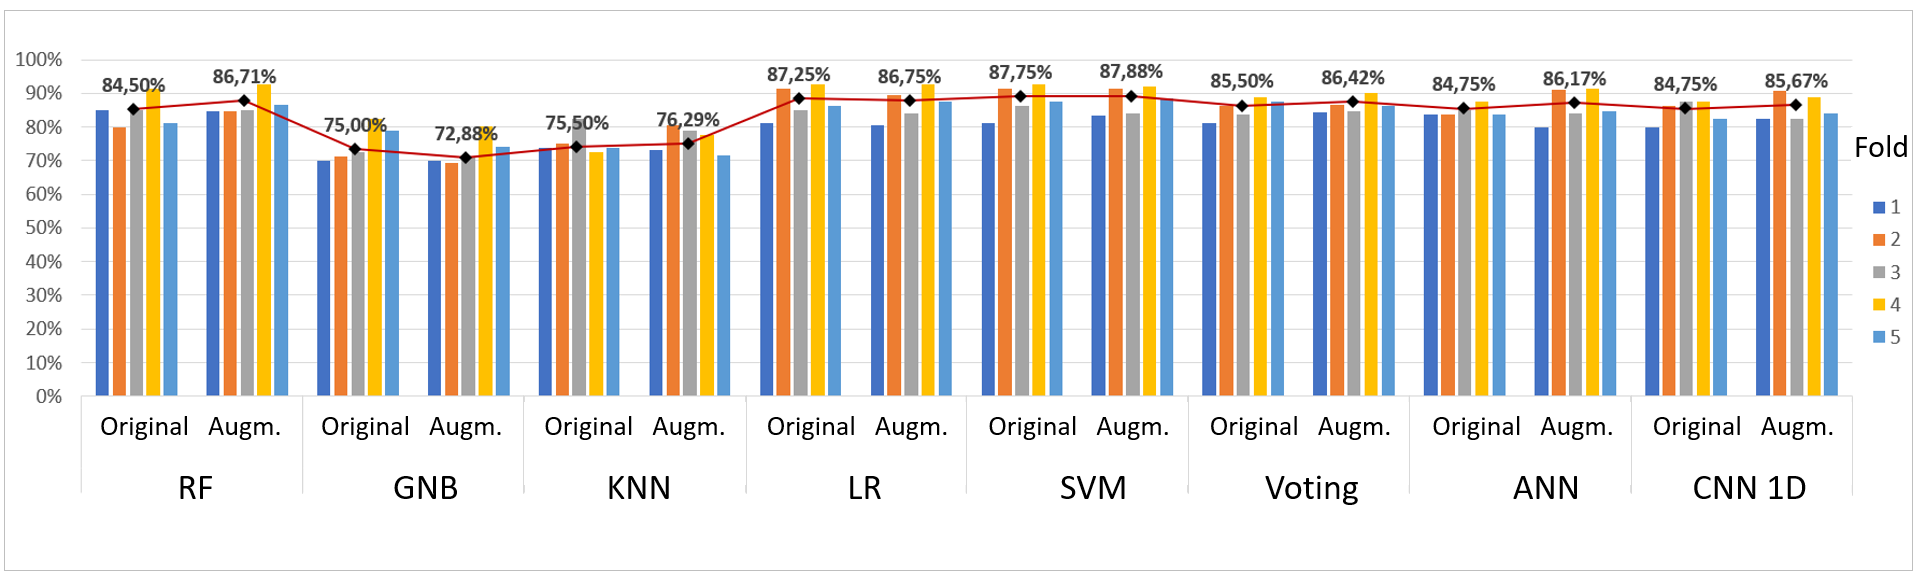
\includegraphics[width=.95\textwidth]{resources/images/060-results/Results_classification_flow_ESC-10_1.png}
        \smallcaption{Source: Author}
        \label{fig:results_ESC-10_classification_results_fold_overview}
\end{figure}


\section{BENCHMARK}
\label{sec:results_metrics}

% Specific objective a) 

This section presents the basic benchmark metrics gathered within the body of literature (Chapter \ref{chp:rel}). Starting with human accuracy, according to \textcite{PiczakESC2015}, an average accuracy rate of 95.7\% was attained for the ESC-10 dataset, while the ESC-50 dataset achieved an accuracy rate of 81.3\%. The recall rates for individual sound event classes displayed significant variation, ranging from 34.1\% for washing machine noise to nearly 100\% for crying babies and barking dogs. These experiments indicate that proficient and attentive listeners have the potential to achieve perfect scores on the smaller dataset and are likely to reach accuracy levels of approximately 90\% on the main dataset, albeit with some uncertainties when categorizing more ambiguous mechanical noises and soundscapes.

To ensure the soundness of the \gls{esr} algorithm, accuracy rates of benchmark datasets were initially compiled from the literature, but only the ones that fully comply with the dataset specifications, more specifically, with k-fold cross-validation setting of 5 for ESC-10, 3 for BDLib2 and 10 for \gls{us8k}. Thus, the values in Table \ref{table:results_benchmark_accuracy} were collected from \textcite{PiczakESC2015}, \textcite{Bountourakis2019}\footnote{The \gls{sti} method better matches the features utilized in this study, with 75.2\% \gls{ann}, 75.0\% \gls{glm}, and 73.6\% \gls{lr}, nevertheless, the highest results were considered in the table.} with the \gls{eti} method,  \textcite{Salamon2014}, and \textcite{Vandendriessche2021}.

\begin{table}[ht!]
    \caption[Benchmark of accuracy rates of the datasets]{Compilation of the accuracy rates to establish a benchmark on the utilized datasets.}
    \label{table:results_benchmark_accuracy}
    \centering
    \begin{tabular}{
        >{\raggedright\arraybackslash}m{0.28\textwidth} | >
        {\centering\arraybackslash}m{0.20\textwidth} | >
        {\centering\arraybackslash}m{0.20\textwidth} | >
        {\centering\arraybackslash}m{0.20\textwidth}}
        \Xhline{2\arrayrulewidth}
        \rowcolor{lightgray}
        \textbf{Classifier} & \textbf{ESC-10} & \textbf{BDLib2} & \textbf{\gls{us8k}}\\
        \hline
        \gls{k-nn}    & 66.7\% & ---    & 56.0\%  \\
        \gls{gnb}     & ---    & ---    & ---     \\
        \gls{svm}     & 67.0\% & ---    & 69.0\%  \\
        \gls{lr}      & ---    & 74.8\% & ---     \\
        \gls{rf}      & 72.7\% & ---    & 66.0\%  \\
        Voting        & ---    & ---    & 10.0\%  \\
        \gls{glm}     & ---    & 80.4\% & ---     \\
        Decision tree & ---    & ---    & 48.0\%  \\
        \gls{ann}     & ---    & 81.5\% & ---     \\
        \gls{cnn} 1D  & 83.2\% & ---    & 60.1\%  \\
     \Xhline{2\arrayrulewidth}
    \end{tabular}
    \smallcaption{Source: Author}
\end{table}

\section{TRAINING AND CLASSIFICATION FLOW}
\label{sec:results_training_classification_flow}

In this initial stage of the experiments, the main objective is to evaluate the \gls{esr} algorithm implemented with several classifiers in terms of feature selection, feature extraction, accuracy, processing memory, flash memory, and response time, in order to select a winning classifier to be used in the next phase. The evaluation was performed using all datasets in a notebook, and subsequently embedded in the Raspberry Pi 4 specifically for the US8K\_AV dataset.

To evaluate the handcrafted feature selection, a Python script was developed to generate various models for k-fold cross-validation. These models included normalization, standardization, normalization + \gls{pca}, and standardization + \gls{pca}. Each model was applied to both the original and augmented datasets. On average, the accuracy rates of the top-performing classifiers increased among the datasets ESC-10 (1.5\%) and BDLib2 (7.4\%) but decreased in the \gls{us8k} (-0.7\%). Notably, as depicted by the colors in Table \ref{table:results_accuracy_overview_classifiers_aug_ori_1}, the winning classifiers were \underline{mostly} the models \textbf{augmented normalized} and \textbf{augmented standardized} for ESC-10 and BDLib2, while for \gls{us8k} were the models \textbf{original normalized} and \textbf{original standardized}. The threshold for the colors was the three highest values and the differences between the exceptions were deemed marginal.

\begin{table}[ht!]
    \caption[Accuracy rates overview using the benchmark datasets - Models augmented x original (Focus on the classifiers line by line)]{Accuracy rates overview using the benchmark datasets - The color difference focuses on the classifiers utilized in the models augmented and original, line by line, with a threshold between the colors for the three highest values.}
    \label{table:results_accuracy_overview_classifiers_aug_ori_1}
     \raggedright
    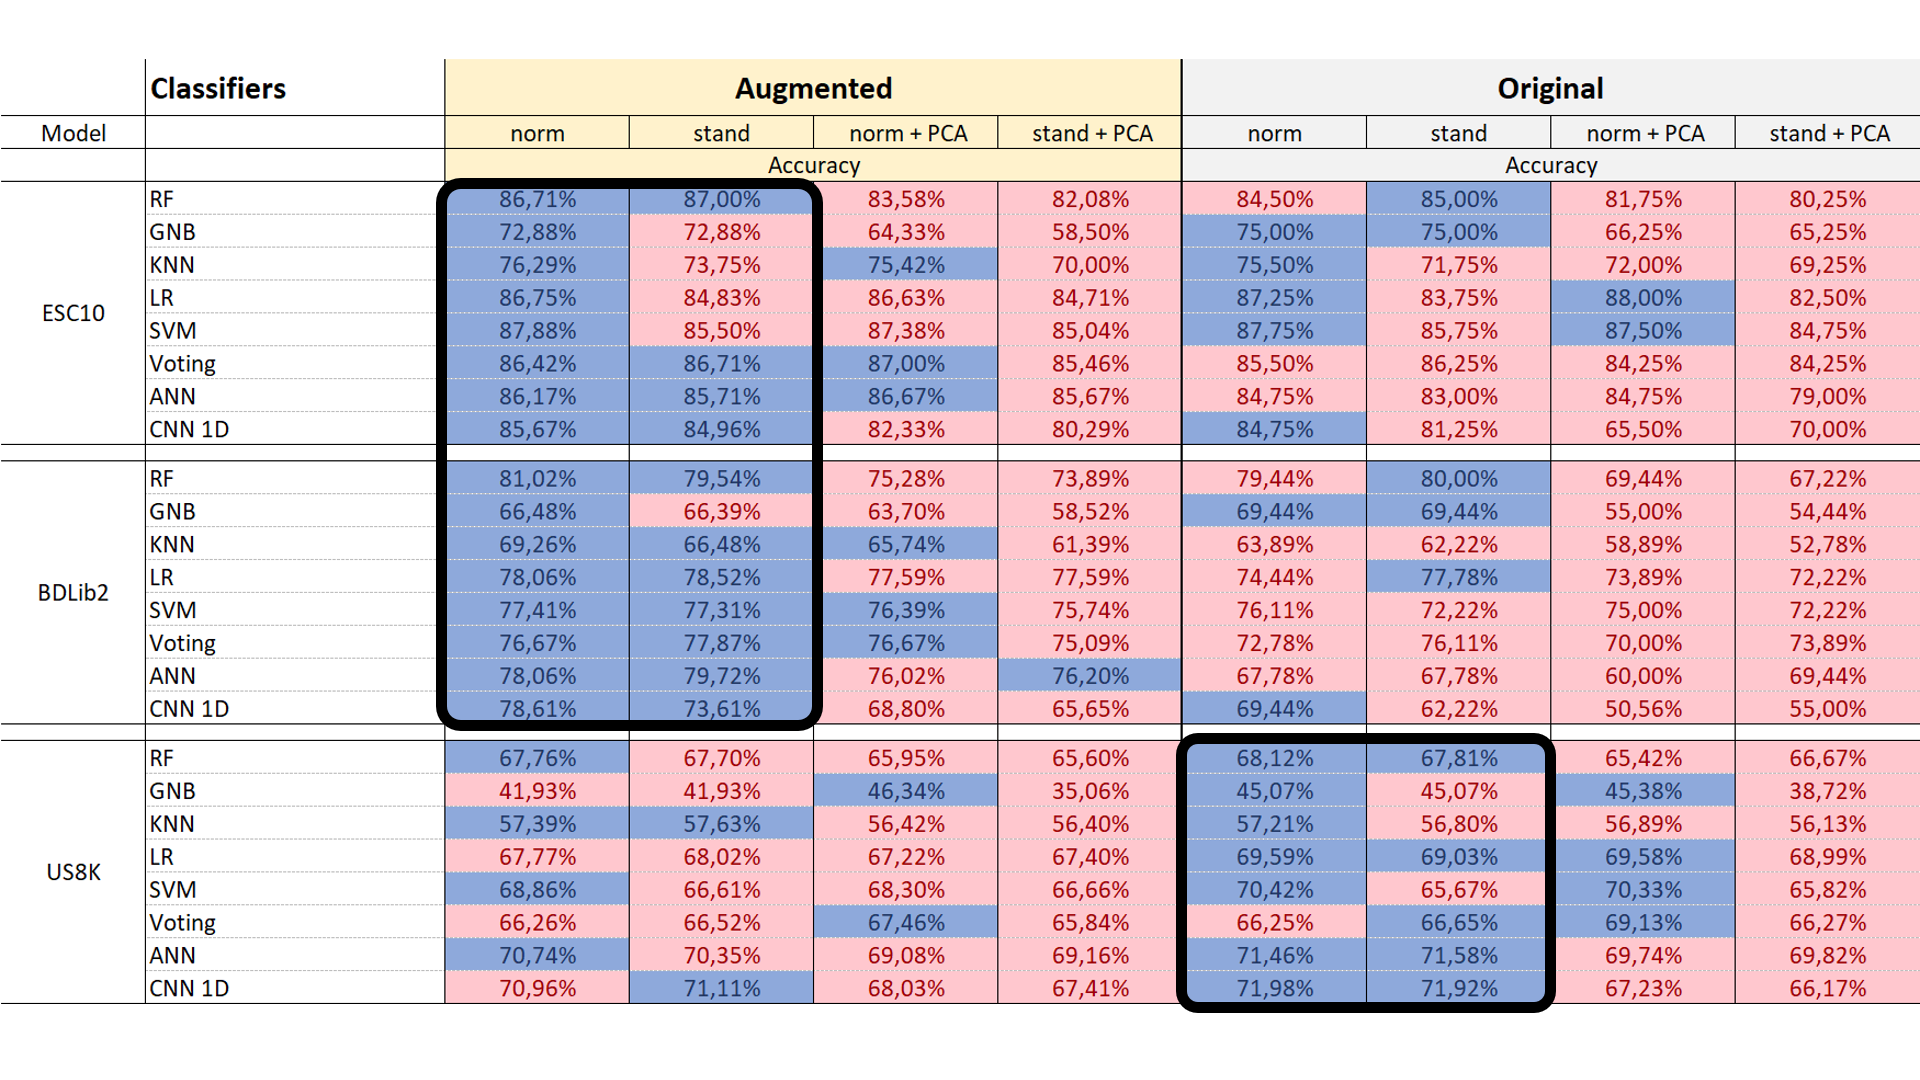
\includegraphics[width=1\textwidth]{resources/images/060-results/Results_classification_overview_aug_x_ori_1.png}
    \smallcaption{Source: Author}
\end{table}

When analyzing the entire datasets with their respective classifiers and models (64 in total), notable performance for the ESC-10 and BDLib2 datasets was observed among classical machine learning techniques, with \textbf{\gls{lr}} and \textbf{\gls{svm}} emerging as the top-performing\footnote{Selected among the models with the highest average accuracy.} along with the ensemble method \textbf{\gls{rf}}. This pattern was not identified in the \gls{us8k}, where the neural networks performed better in every model, more specifically, in the normalized and standardized models. Consistently, the same behavior from classifier by classifier emerged in the dataset by dataset, wherein models \textbf{augmented} for ESC-10 and BDLib2 and \textbf{original} for \gls{us8k} yielded the \underline{majority of best results}, as illustrated by the color difference in Table \ref{table:results_accuracy_overview_classifiers_aug_ori_2} with a 20\% threshold for the highest values.

\begin{table}[ht!]
    \caption[Accuracy rates overview using the benchmark datasets - Models augmented x original (Focus on the classifiers dataset by dataset)]{Accuracy rates overview using the benchmark datasets - The color difference focuses on the classifiers utilized in the models augmented and original, dataset by dataset, with a 20\% threshold between the colors for the highest values.}
    \label{table:results_accuracy_overview_classifiers_aug_ori_2}
     \raggedright
    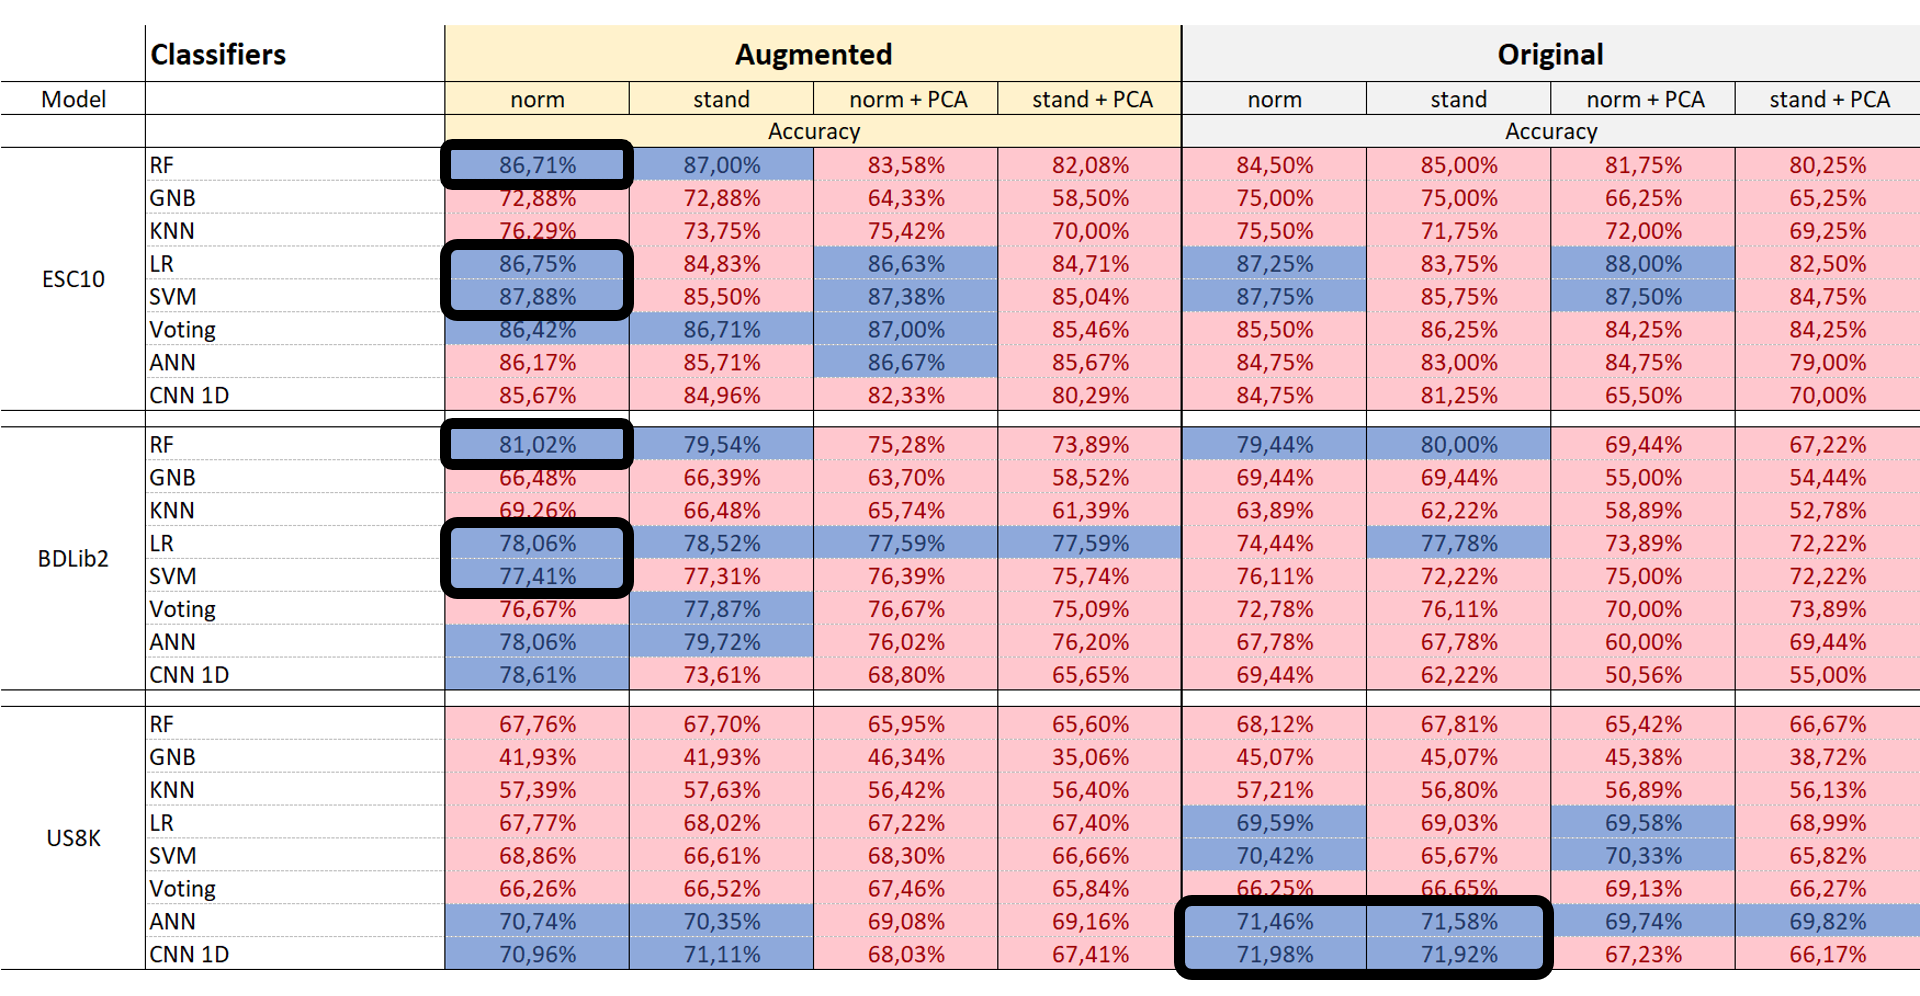
\includegraphics[width=1\textwidth]{resources/images/060-results/Results_classification_overview_aug_x_ori_2.png}
    \smallcaption{Source: Author}
\end{table}

After analyzing the feature extraction process with a single window, the same process was repeated with a sliding window of 1 \gls{s}, sampling rate of 22,050 \gls{hz}, and 50\% overlapping between windows. The accuracy across all datasets exhibited an approximate \underline{5\% decline}, as evidenced in Table \ref{table:results_accuracy_overview_features_windowed} by the color difference among the classifiers, line by line, with a
threshold between the colors for the three highest values. This result aligns well with the findings from \textcite{Salamon2014}, wherein both classifiers \gls{svm} and \gls{rf} also had a decrease in accuracy of around 5\% (graphically estimated) when transitioning from 4 \gls{s} to 1 \gls{s} audio slices. 

\begin{table}[ht!]
    \caption[Accuracy rates overview using the benchmark datasets - Models augmented x windowed (Focus on the classifiers line by line)]{Accuracy rates overview using the benchmark datasets - The color difference focuses on the classifiers utilized in the models augmented and windowed, line by line, with a threshold between the colors for the three highest values.}
    \label{table:results_accuracy_overview_features_windowed}
     \raggedright
    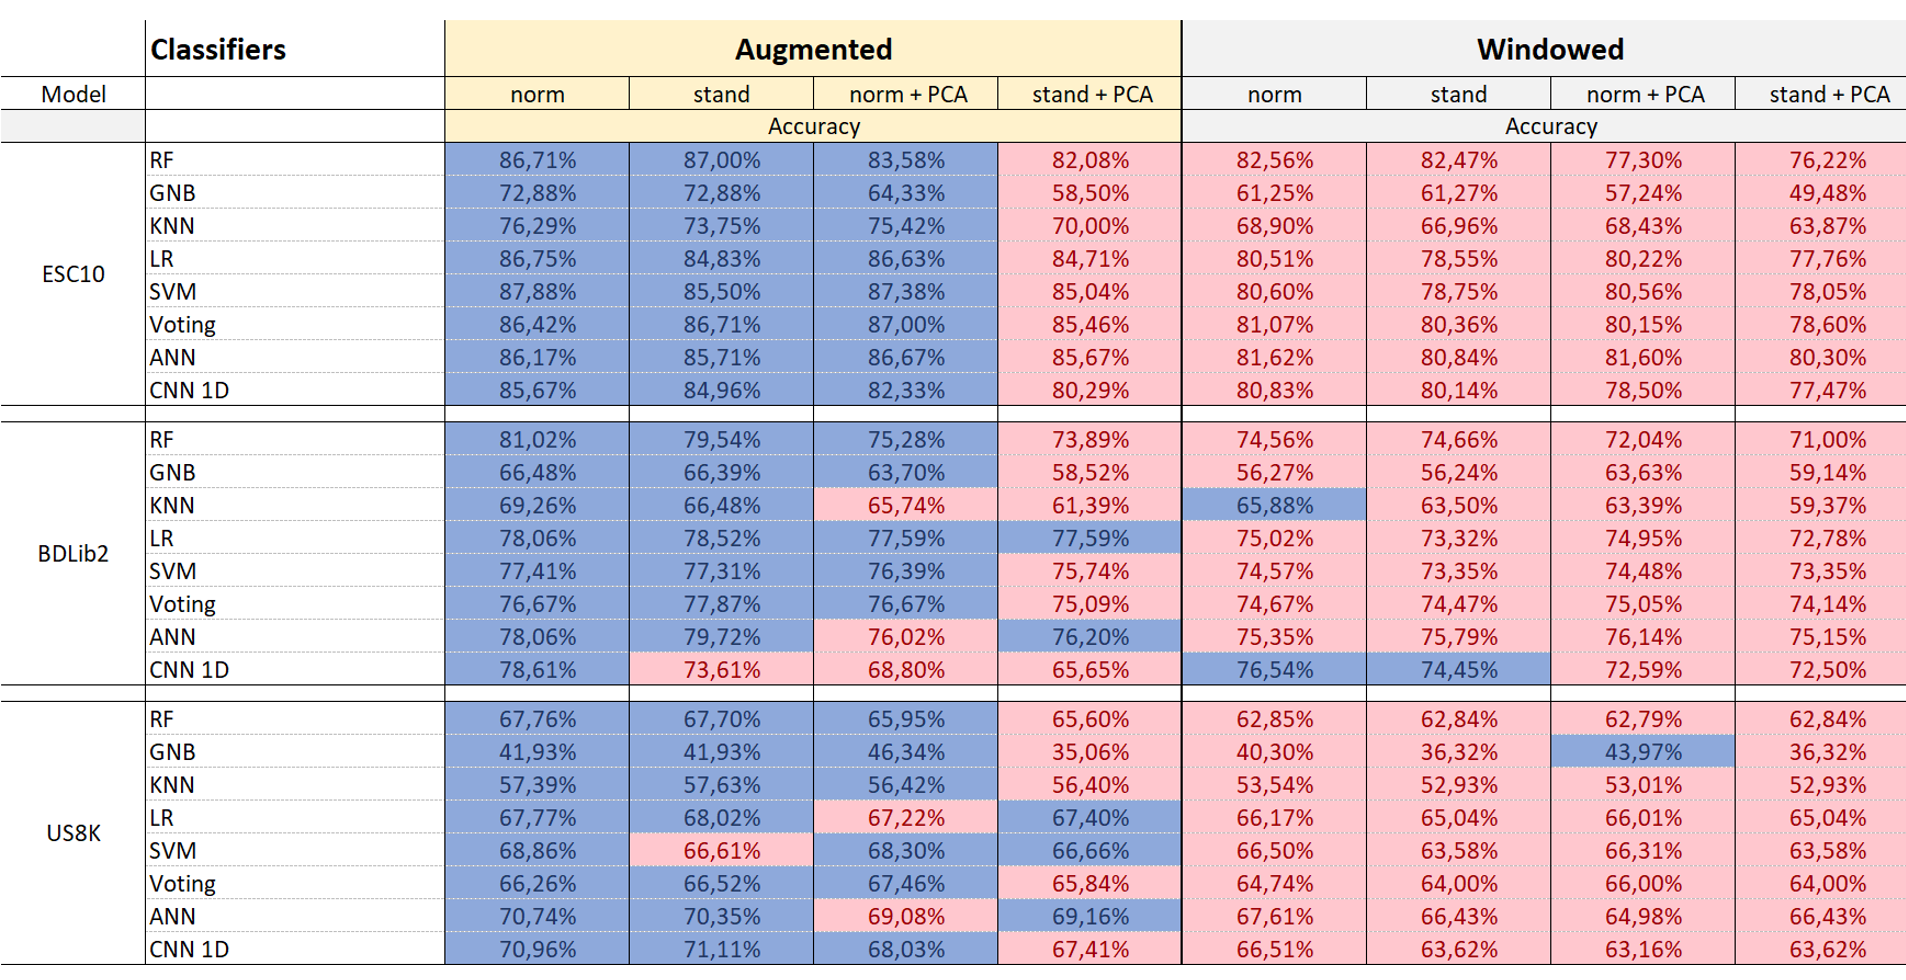
\includegraphics[width=1\textwidth]{resources/images/060-results/Results_classification_overview_aug_x_ori_3.png}
    \smallcaption{Source: Author}
\end{table}

At this point, the benchmark Table \ref{table:results_benchmark_accuracy} was updated with the best accuracy rates from Table \ref{table:results_accuracy_overview_classifiers_aug_ori_2}. The comparison is presented in Table \ref{table:results_accuracy_comparison}, and it entails that the feature selection was sound overcoming all rates of comparable classifiers except by the \gls{ann} in the BDLib2 dataset.

\begin{table}[ht!]
    \caption[Comparison of the accuracy rates benchmark with the best models from cross-validation]{Compilation of the benchmark (BM) of accuracy rates against the augmented normalized models for ESC-10 and BDLib2 and original normalized models for \gls{us8k}.}
    \label{table:results_accuracy_comparison}
    \centering
    \begin{tabular}{
        >{\raggedright\arraybackslash}m{0.15\textwidth} | >
        {\centering\arraybackslash}m{0.10\textwidth} | >
        {\columncolor{lime}\centering\arraybackslash}m{0.12\textwidth} | >
        {\centering\arraybackslash}m{0.10\textwidth} | >
        {\columncolor{lime}\centering\arraybackslash}m{0.12\textwidth} | >
        {\centering\arraybackslash}m{0.10\textwidth} | >       
        {\columncolor{lime}\centering\arraybackslash}m{0.11\textwidth}}
        \Xhline{2\arrayrulewidth}
        \rowcolor{lightgray}
        \textbf{Classifier} & \textbf{ESC-10} & \textbf{ESC-10} & \textbf{BDLib2} & \textbf{BDLib2} & \textbf{US8K} & \textbf{US8K} \\
        \rowcolor{lightgray}
        & BM & Aug. norm & BM & Aug. norm & BM & Ori. norm \\
        \hline
        k-NN            & 66.7\% & 76.3\% & ---    & 69.3\% & 56.0\% & 57.2\%   \\
        GNB             & ---    & 72.9\% & ---    & 66.5\% & ---    & 45.1\%   \\
        SVM             & 67.0\% & 87.9\% & ---    & 77.4\% & 69.0\% & 70.4\%   \\
        LR              & ---    & 86.8\% & 74.8\% & 78.1\% & ---    & 69.6\%   \\
        RF              & 72.7\% & 86.7\% & ---    & 81.0\% & 66.0\% & 68.1\%   \\
        Voting          & ---    & 86.4\% & ---    & 76.7\% & 10.0\% & 71.5\%   \\
        GLM             & ---    & ---    & 80.4\% & ---    & ---    & ---      \\
        Decision tree   & ---    & ---    & ---    & ---    & 48.0\% & ---      \\
        ANN             & ---    & 86.2\% & \cellcolor{lime}81.5\% & \cellcolor{white} 78.1\% & --- & 71.5\%   \\
        CNN 1D          & 83.2\% & 85.7\% & ---    & 78.6\% & 60.1\% & 72.0\%   \\          
    \Xhline{2\arrayrulewidth}
    \end{tabular}
    \smallcaption{Source: Author}
\end{table}


% Specific objective b).

The dataset created in subsection \ref{subsec:dataset_US8K_AV}, referred to as US8K\_AV, consists of 4,908 files distributed across 6 classes. These files collectively represent a total duration of 4.94 hours of recorded sounds. To maintain consistency and facilitate accuracy comparisons, the original 10-fold split for cross-validation from the source dataset (\gls{us8k}) was retained.

Similarly to the \gls{us8k} dataset, the augmentation process resulted in a slight decline in accuracy rates for the top-performing classifiers among the machine learning techniques, whereas the neural network models exhibited a marginal improvement (Table \ref{table:results_accuracy_overview_us8k_av_aug_ori_1}, upper area). Given the time-consuming effort required for training the augmented model and the substantial increase in the size of the feature model subsequently, there appears to be no practical justification for adopting augmentation techniques within this tailored dataset.

Considering the original normalized model, \textbf{\gls{svm}} and \textbf{\gls{ann}} outperformed the other classifiers, achieving an average accuracy of 83\%. These were followed by \textbf{\gls{lr}} and \textbf{\gls{cnn} 1D}, both attaining an accuracy of 82\%. Notably, \gls{ann} demonstrated the highest stability among the models, with its accuracy consistently ranging between 82\% and 83\%. A comparable pattern emerged in the windowed normalized models (Table \ref{table:results_accuracy_overview_us8k_av_aug_ori_1}, lower area — for emphasis, only windowed models were colored), with the same four classifiers ranked as top-performing. However, the sliding window process introduced the same overhead noticed in the other datasets, reducing the average accuracy by 5\%, ranging now between 77\% and 79\%.

\begin{table}[ht!]
    \caption[Accuracy rates overview using the tailored dataset US8K\_AV.]{Accuracy rates overview of the best models using the tailored dataset US8K\_AV. The color difference focuses on the classifiers utilized in the models, dataset by dataset, with a 20\% threshold between the colors for the highest values.}
    \label{table:results_accuracy_overview_us8k_av_aug_ori_1}
     \raggedright
    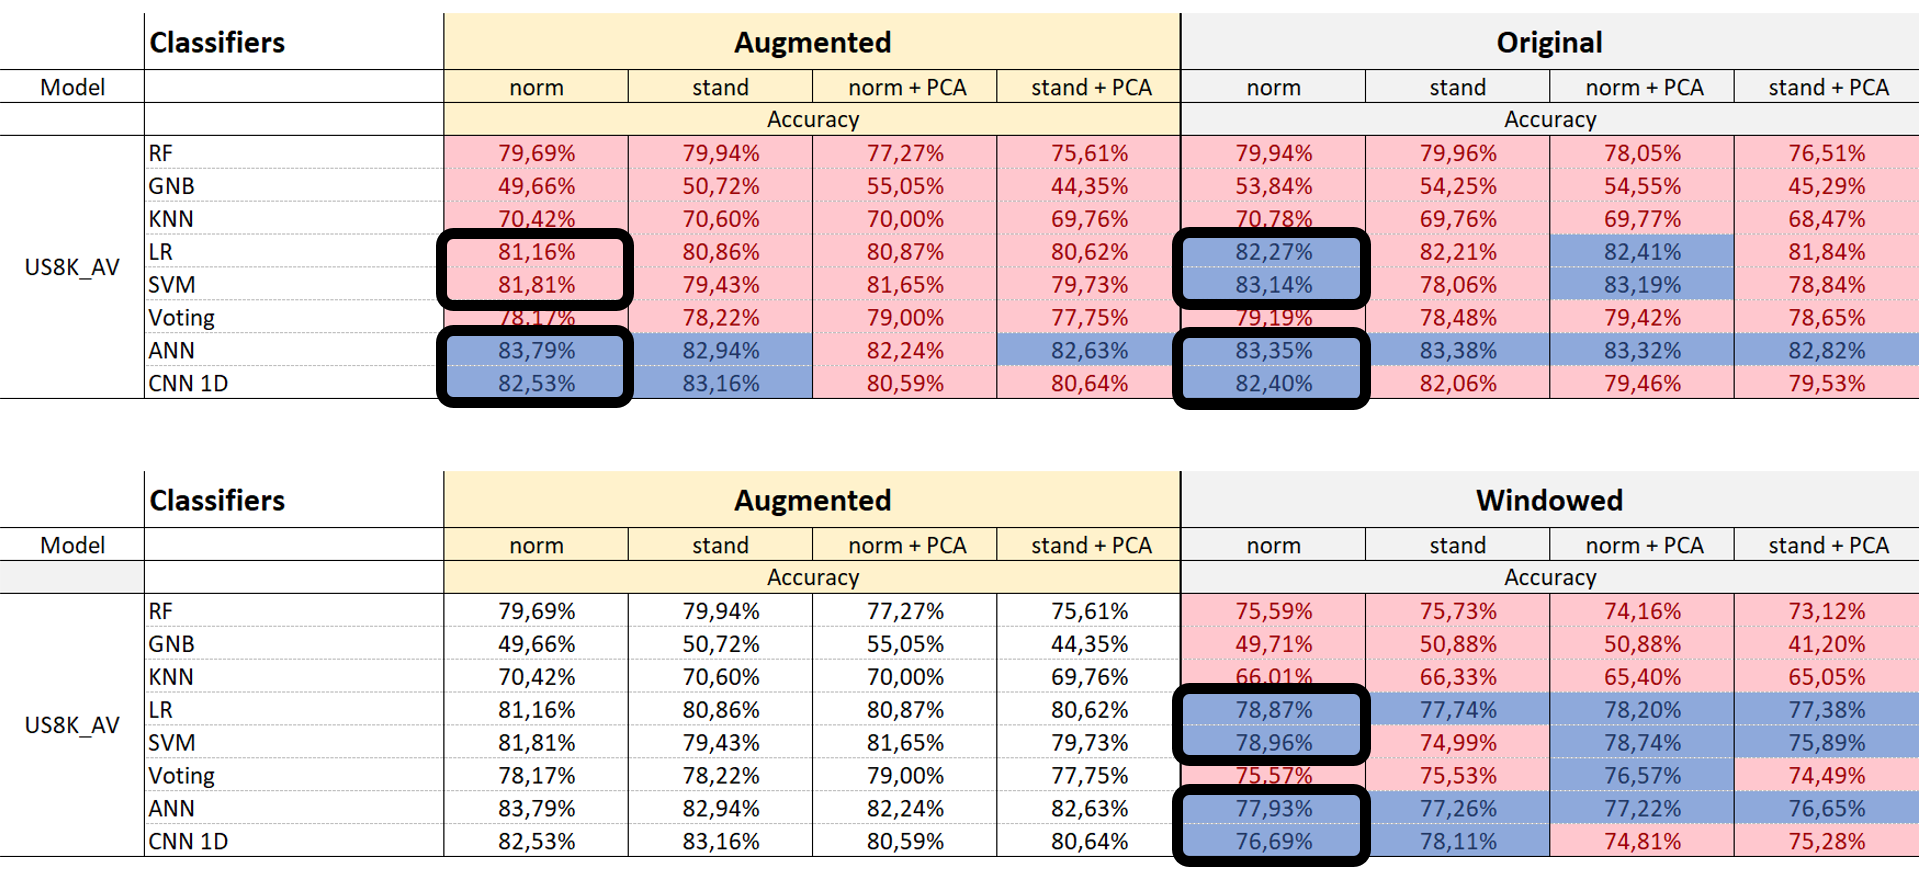
\includegraphics[width=1\textwidth]{resources/images/060-results/Results_classification_overview_us8k_av_aug_x_ori_1.png}
    \smallcaption{Source: Author}
\end{table}

%The $t$\_statistic` specifically quantifies the difference between the means of these two groups, normalized by the variability of their differences. It serves as an indicator of whether there is a statistically significant difference between the two sets of accuracy measurements. A higher absolute value of $t$\_statistic suggests a greater likelihood that the observed difference is not due to random chance.

To finalize the evaluation of the feature extraction process, the aforementioned 5\% reduction in accuracy between the augmented and windowed models was statistically evaluated with paired samples $t$-test using the results plotted in Table \ref{table:results_accuracy_overview_features_windowed} and Table \ref{table:results_accuracy_overview_us8k_av_aug_ori_1}. The hypotheses for this evaluation were formulated as follows:

\begin{itemize}
    \item Null hypothesis ($H_0$): There is no significant difference between the performance of the augmented model and the windowed model;
    \item Alternative hypothesis ($H_a$): There is a significant difference between the performance of the augmented model and the windowed model.
\end{itemize}

Given the $p$-value = 0.005, the null hypothesis was rejected in all datasets, as illustrated in Table \ref{table:results_paired_t-test_datasets}, and therefore, there is a statistically significant difference in performance between the augmented and windowed models within the datasets and classifiers analyzed. This pattern was also observed across classifiers among the datasets, albeit with a higher probability ($p$-value = 0.05) and with \gls{gnb} as the exception (Table \ref{table:results_paired_t-test_classifiers}).

%This result is not conclusive; rather, it provides evidence that needs to be consistently observed and replicated in further studies to identify a reliable trend.

\begin{table}[ht!]
    \caption[Statistic evaluation of the accuracy rates between the augmented and windowed models among datasets]{Statistic evaluation of the accuracy rates between the augmented and windowed models among datasets.}
    \label{table:results_paired_t-test_datasets}
    \centering
    \begin{tabular}{
        >{\arraybackslash}m{0.30\textwidth} | >
        {\centering\arraybackslash}m{0.30\textwidth} | >
        {\centering\arraybackslash}m{0.30\textwidth}}
        \Xhline{2\arrayrulewidth}
        \rowcolor{lightgray}
        \textbf{Dataset} & \textbf{$t$-test statistic} & \textbf{$p$-value}\\
        \hline
            BDLib2      & 4.064637      & 0.004781 \\
            ESC-10      & 7.491015      & 0.000138 \\
            \gls{us8k}  & 6.106191      & 0.000488 \\
            US8K\_AV    & 4.974953      & 0.001610 \\
     \Xhline{2\arrayrulewidth}
    \end{tabular}
    \smallcaption{Source: Author}
\end{table}


\begin{table}[ht!]
    \caption[Statistic evaluation of the accuracy results between the augmented and windowed models among classifiers]{Statistic evaluation of the accuracy results between the augmented and windowed models among classifiers.}
    \label{table:results_paired_t-test_classifiers}
    \centering
    \begin{tabular}{
        >{\arraybackslash}m{0.30\textwidth} | >
        {\centering\arraybackslash}m{0.30\textwidth} | >
        {\centering\arraybackslash}m{0.30\textwidth}}
        \Xhline{2\arrayrulewidth}
        \rowcolor{lightgray}
        \textbf{Classifier} & \textbf{$t$-test statistic} & \textbf{$p$-value}\\
        \hline
            \gls{rf}     & 8.872540       & 0.003019 \\
            \gls{gnb}    & 1.977806       & 0.142361 \\
            \gls{k-nn}   & 5.265241       & 0.013351 \\
            \gls{lr}     & 3.211662       & 0.048894 \\
            \gls{svm}    & 3.320547       & 0.045036 \\
            Voting       & 3.346427       & 0.044176 \\
            \gls{ann}    & 5.679546       & 0.010816 \\
            \gls{cnn} 1D & 5.378761       & 0.012585 \\
     \Xhline{2\arrayrulewidth}
    \end{tabular}
    \smallcaption{Source: Author}
\end{table}


% Specific objective c).

All steps used in the previous process with handcrafted features were now repeated using aggregated features. For simplification and given the results presented thus far, only the results from the dataset US8K\_AV were reported.

During the training of the \gls{cnn} 2D models, the architecture that demonstrated the best performance for the sliding window process was adapted from \textcite{Su2020}, achieving an average accuracy of 80\% with 1.5 million trainable parameters. This model also presented a decrease in accuracy between the augmented and windowed models (statistically confirmed across folds with paired sample $t$-test and $p$-value < 0.05). Notably, the model adapted from \textcite{Luz2021} had fewer trainable parameters (200,000) and attained the highest score (86\%) in the single window process. However, it exhibited a significant drop in accuracy during the sliding window process, decreasing to 77\%, as shown in Table \ref{table:results_accuracy_overview_us8k_av_cnn_2D}. This pattern was consistently observed across all datasets, including a modest improvement in average accuracy resulting from the augmentation process, which was not identified in the previous classifiers. Due to resource limitations and low trade-offs, the windowed augmented model was not investigated.

\begin{table}[ht!]
    \caption[Accuracy rates for each fold of the tailored dataset US8K\_AV.]{Accuracy rates for each fold of the tailored dataset US8K\_AV, models original and augmented, both using two different architectures.}
    \label{table:results_accuracy_overview_us8k_av_cnn_2D}
     \raggedright
    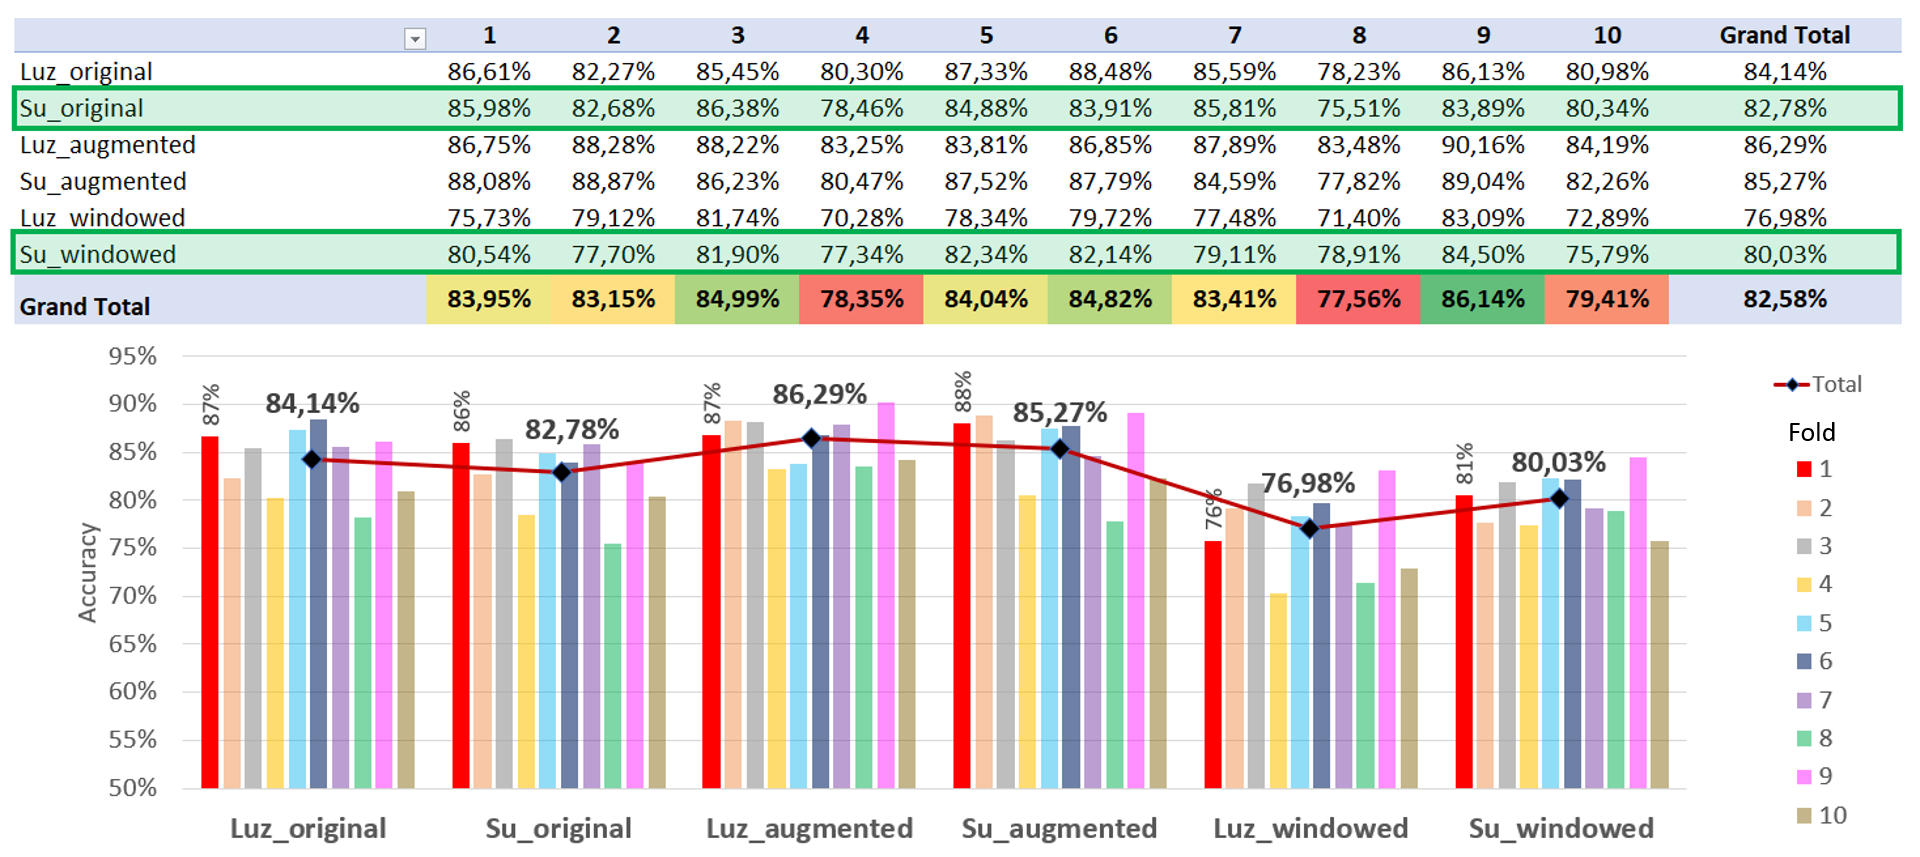
\includegraphics[width=1\textwidth]{resources/images/060-results/Results_classification_overview_us8k_av_cnn2d.png}
    \smallcaption{Source: Author}
\end{table}


At this moment, the following outcomes were identified and will henceforth be adopted:
\begin{itemize}
    \item Models utilizing handcrafted features will be normalized. The processes of standardization and \gls{pca} will no longer be considered for these models;
    \item The augmentation process has been observed to enhance the performance of \gls{cnn} 2D models across all datasets, however, it will not be applied in the windowed model for the US8K\_AV dataset;
    \item A comprehensive benchmark for the US8K\_AV dataset has been established with top-performing classifiers using k-fold cross-validation accuracy metrics (Table \ref{table:results_feature_extraction_and_classifiers_us8k_av}). This benchmark includes:
    \begin{itemize}
        \item Machine learning techniques employing handcrafted features: \textbf{\gls{svm}} and \textbf{\gls{lr}};
        \item Neural networks utilizing handcrafted features: \textbf{\gls{ann}} and \textbf{\gls{cnn} 1D};
        \item Neural networks utilizing aggregated features: \textbf{\gls{cnn} 2D}.
    \end{itemize}
    \item \textbf{\gls{rf}} has been incorporated into the benchmark to represent the results involving ensemble methods;
    \item Only \textbf{windowed models} will be considered to minimize the full prediction time.
\end{itemize}


\begin{table}[ht!]
    \caption[Benchmark of accuracy rates for the dataset US8K\_AV.]{Compilation of the feature extraction processes and top-performing classifiers on the US8K\_AV dataset.}
    \label{table:results_feature_extraction_and_classifiers_us8k_av}
    \centering
    \begin{tabular}{
        >{\arraybackslash}m{0.30\textwidth} | >
        {\centering\arraybackslash}m{0.30\textwidth} | >
        {\centering\arraybackslash}m{0.30\textwidth}}
        \Xhline{2\arrayrulewidth}
        \rowcolor{lightgray}
        \textbf{Features - Classifier} & \textbf{Sliding window (1 s)} & \textbf{Single window (4 s)}\\
        \rowcolor{lightgray}
        \rowcolor{lightgray}
         &  Acc. (Std) & Acc. (Std)   \\
        \hline
        Handcrafted - \gls{svm}    & 78.96\% \hspace{0.5cm} (1.82\%) & 
                                     83.14\% \hspace{0.5cm} (2.21\%)\\
        Handcrafted - \gls{lr}     & 78.87\% \hspace{0.5cm} (1.49\%) & 
                                     82.27\% \hspace{0.5cm} (2.74\%)\\
        Handcrafted - \gls{rf}     & 75.59\% \hspace{0.5cm} (2.72\%) & 
                                     79.94\% \hspace{0.5cm} (2.63\%)\\
        Handcrafted - \gls{ann}    & 77.93\% \hspace{0.5cm} (3.29\%) & 
                                     83.35\% \hspace{0.5cm} (2.91\%)\\
        Handcrafted - \gls{cnn} 1D & 76.69\% \hspace{0.5cm} (3.74\%) & 
                                     82.40\% \hspace{0.5cm} (2.72\%)\\
        Aggregated - \gls{cnn} 2D  & 80.03\% \hspace{0.5cm} (2.71\%) & 
                                     82.78\% \hspace{0.5cm} (3.60\%)\\
     \Xhline{2\arrayrulewidth}
    \end{tabular}
    \smallcaption{Source: Author}
\end{table}

Upon completing the training and classification flow, the next step involves deploying the \underline{top-performing classifiers of the US8K\_AV dataset to the Raspberry Pi} and evaluating its performance in terms of accuracy and real-time processing capabilities. However, before proceeding, several definitions must be established. A 'predictive model' refers to a trained classifier saved as a pickle file (.PKL) for \gls{svm}, \gls{lr}, and \gls{rf} or as an .HDF5 file for neural networks such as \gls{ann}, \gls{cnn} 1D, and \gls{cnn} 2D. The term 'predictive algorithm' or '\gls{esr} algorithm' encompasses the necessary functions to record live audio, extract features, feed them into the predictive model, and return the inference as a single class.

The 'response time' or 'total prediction time' is defined as the aggregate duration of the individual operations involved in the predictive algorithm. The time required for feature extraction denotes the duration necessary to extract features according to the specified method (handcrafted or aggregated). The average time required by the predictive model to perform sound classification using the feature vectors from all frames is referred to as classification time. Therefore, the total prediction time corresponds to the sum of the feature extraction process and the classification time. However, it does not account for the time required to digitize the audio, which will be involved in the 'full prediction time' corresponding to the sum of this digitization time and the total prediction time.

'Processing memory', particularly \gls{ram}, serves as a critical component in the predictive algorithm, facilitating the rapid storage and retrieval of data necessary for real-time audio signal processing involving the initial stages of sound capture, feature extraction, loading the predictive model, and performing the classification tasks.

The predictive models were trained using folds 2 through 10, reserving fold 1 as the testing set. This decision was initially substantiated using the \gls{cnn} 2D model (Su windowed) from Table \ref{table:results_accuracy_overview_us8k_av_cnn_2D}, which indicated that fold 1 was among the top five folds across all architectural models. Additionally, fold 1 exhibited an accuracy of 80.54\%, closely aligning with the result of the 10-fold cross-validation (80.03\%). The same analysis was then performed on the remaining top-performing classifiers, confirming fold 1 as the testing set and resulting in an average accuracy among the models ranging from 77.08\% to 81.71\%, as shown in the confusion matrices of Figure \ref{fig:Results_models_evaluation}. Anticipating the necessity to deploy the neural network models, the predictive models for \gls{ann}, \gls{cnn} 1D, and \gls{cnn} 2D underwent a quantization process using TensorFlow Lite (TFLite) with standard parameters. Notably, there was no significant decline in accuracy following this process, with the results now ranging from 77.08\% to 80.57\% (Figure \ref{fig:Results_nn_models_evaluation}). The projected average confidence interval based on k-fold cross-validation is 0.23\% given a confidence level of 99\%.

\begin{figure}[htbp]
    \raggedright
        \caption{Accuracy evaluation of the predictive models.}
        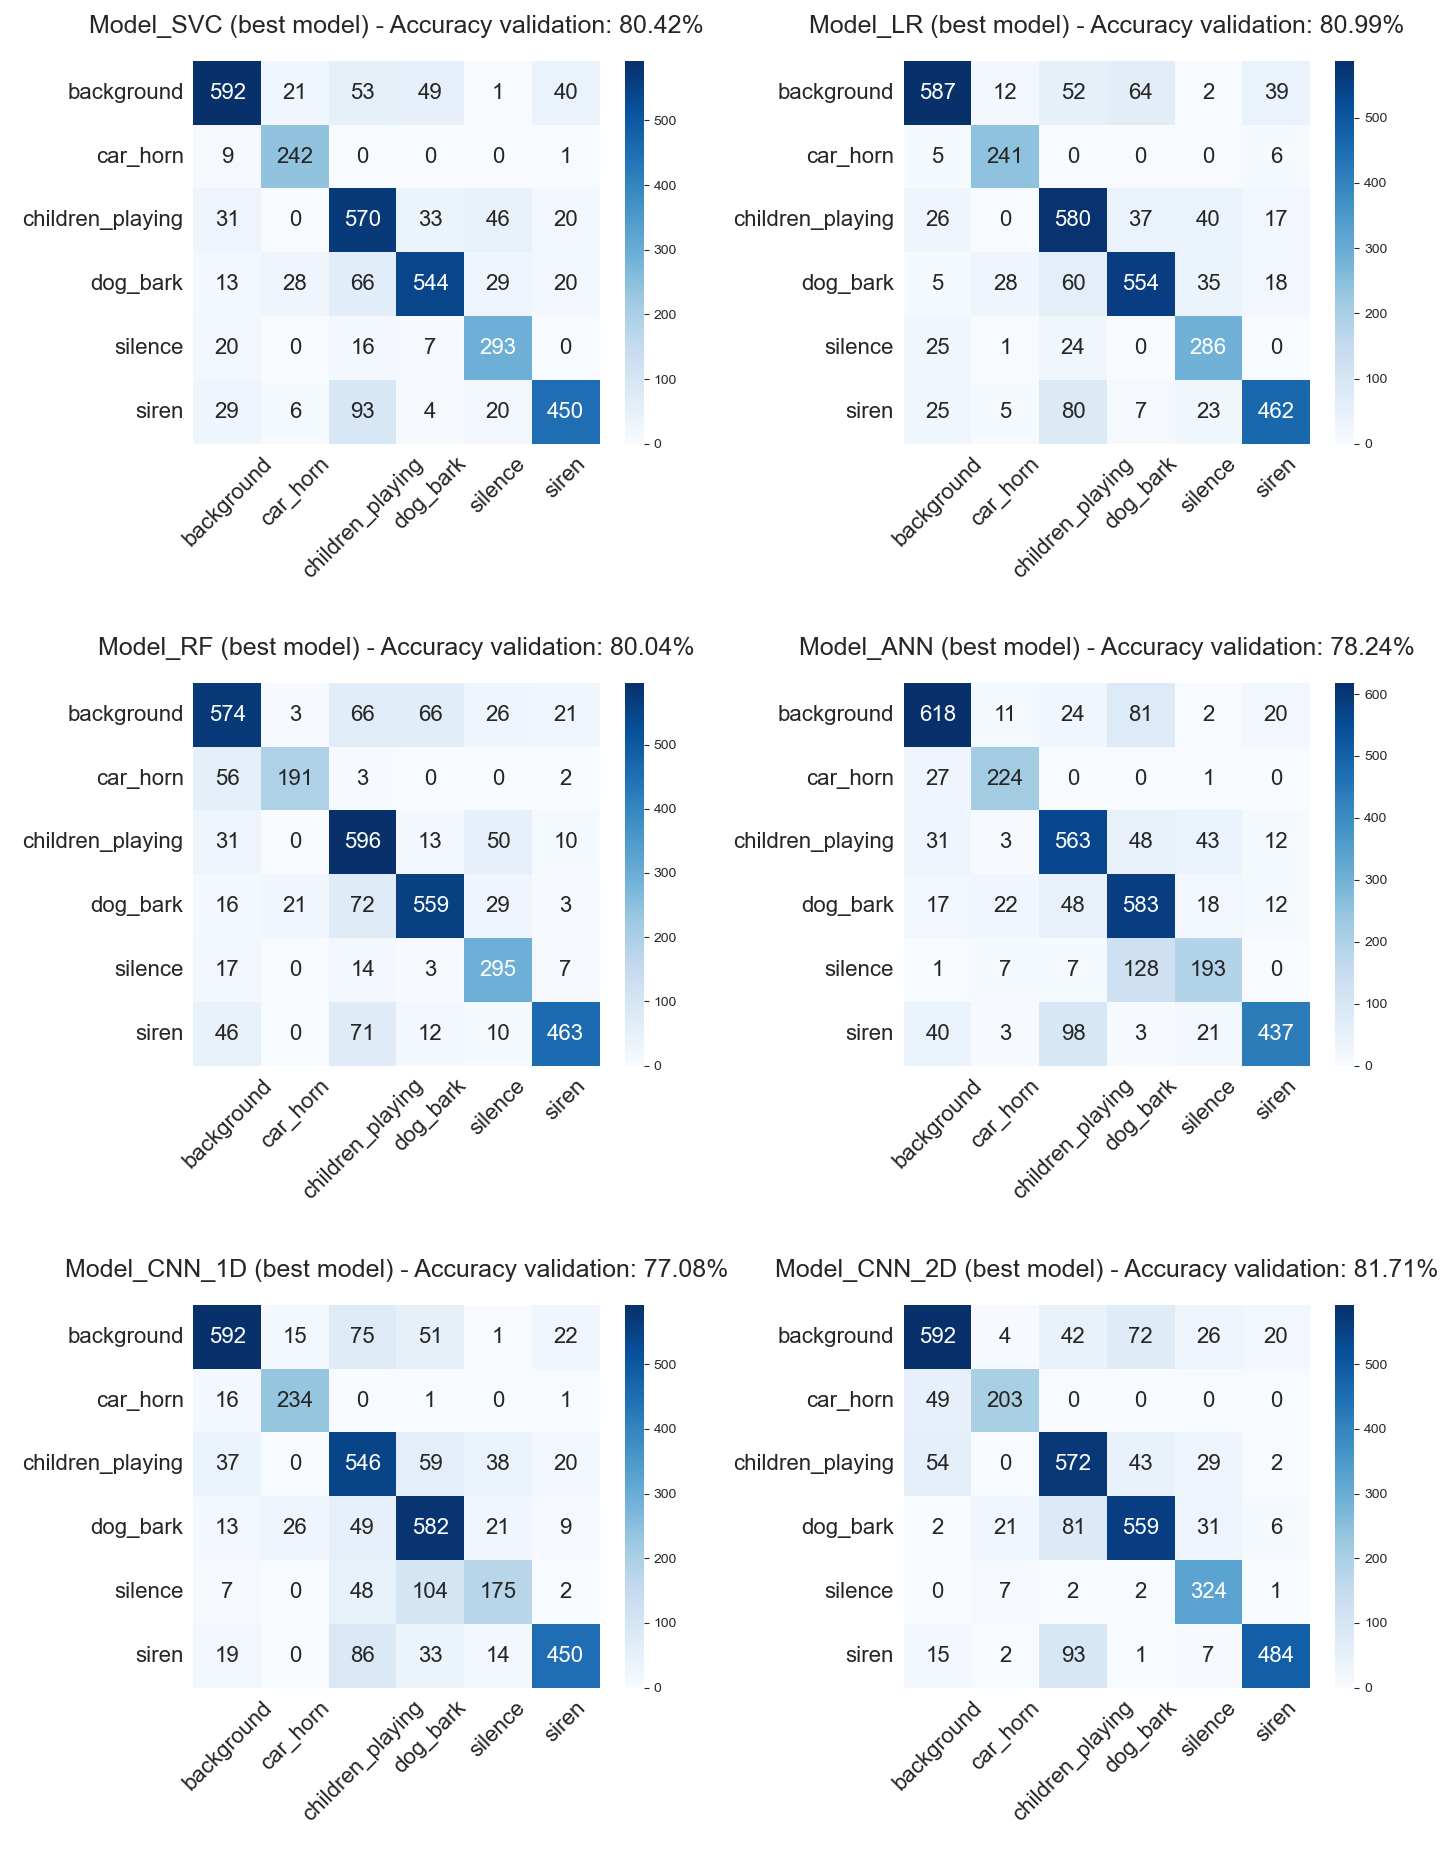
\includegraphics[width=1\textwidth]{resources/images/060-results/Results_classification_overview_models_evaluation_1.png}
        \smallcaption{Source: Author}
        \label{fig:Results_models_evaluation}
\end{figure}

\begin{figure}[htbp]
    \raggedright
        \caption{Accuracy evaluation of the neural network models after the quantization process.}
        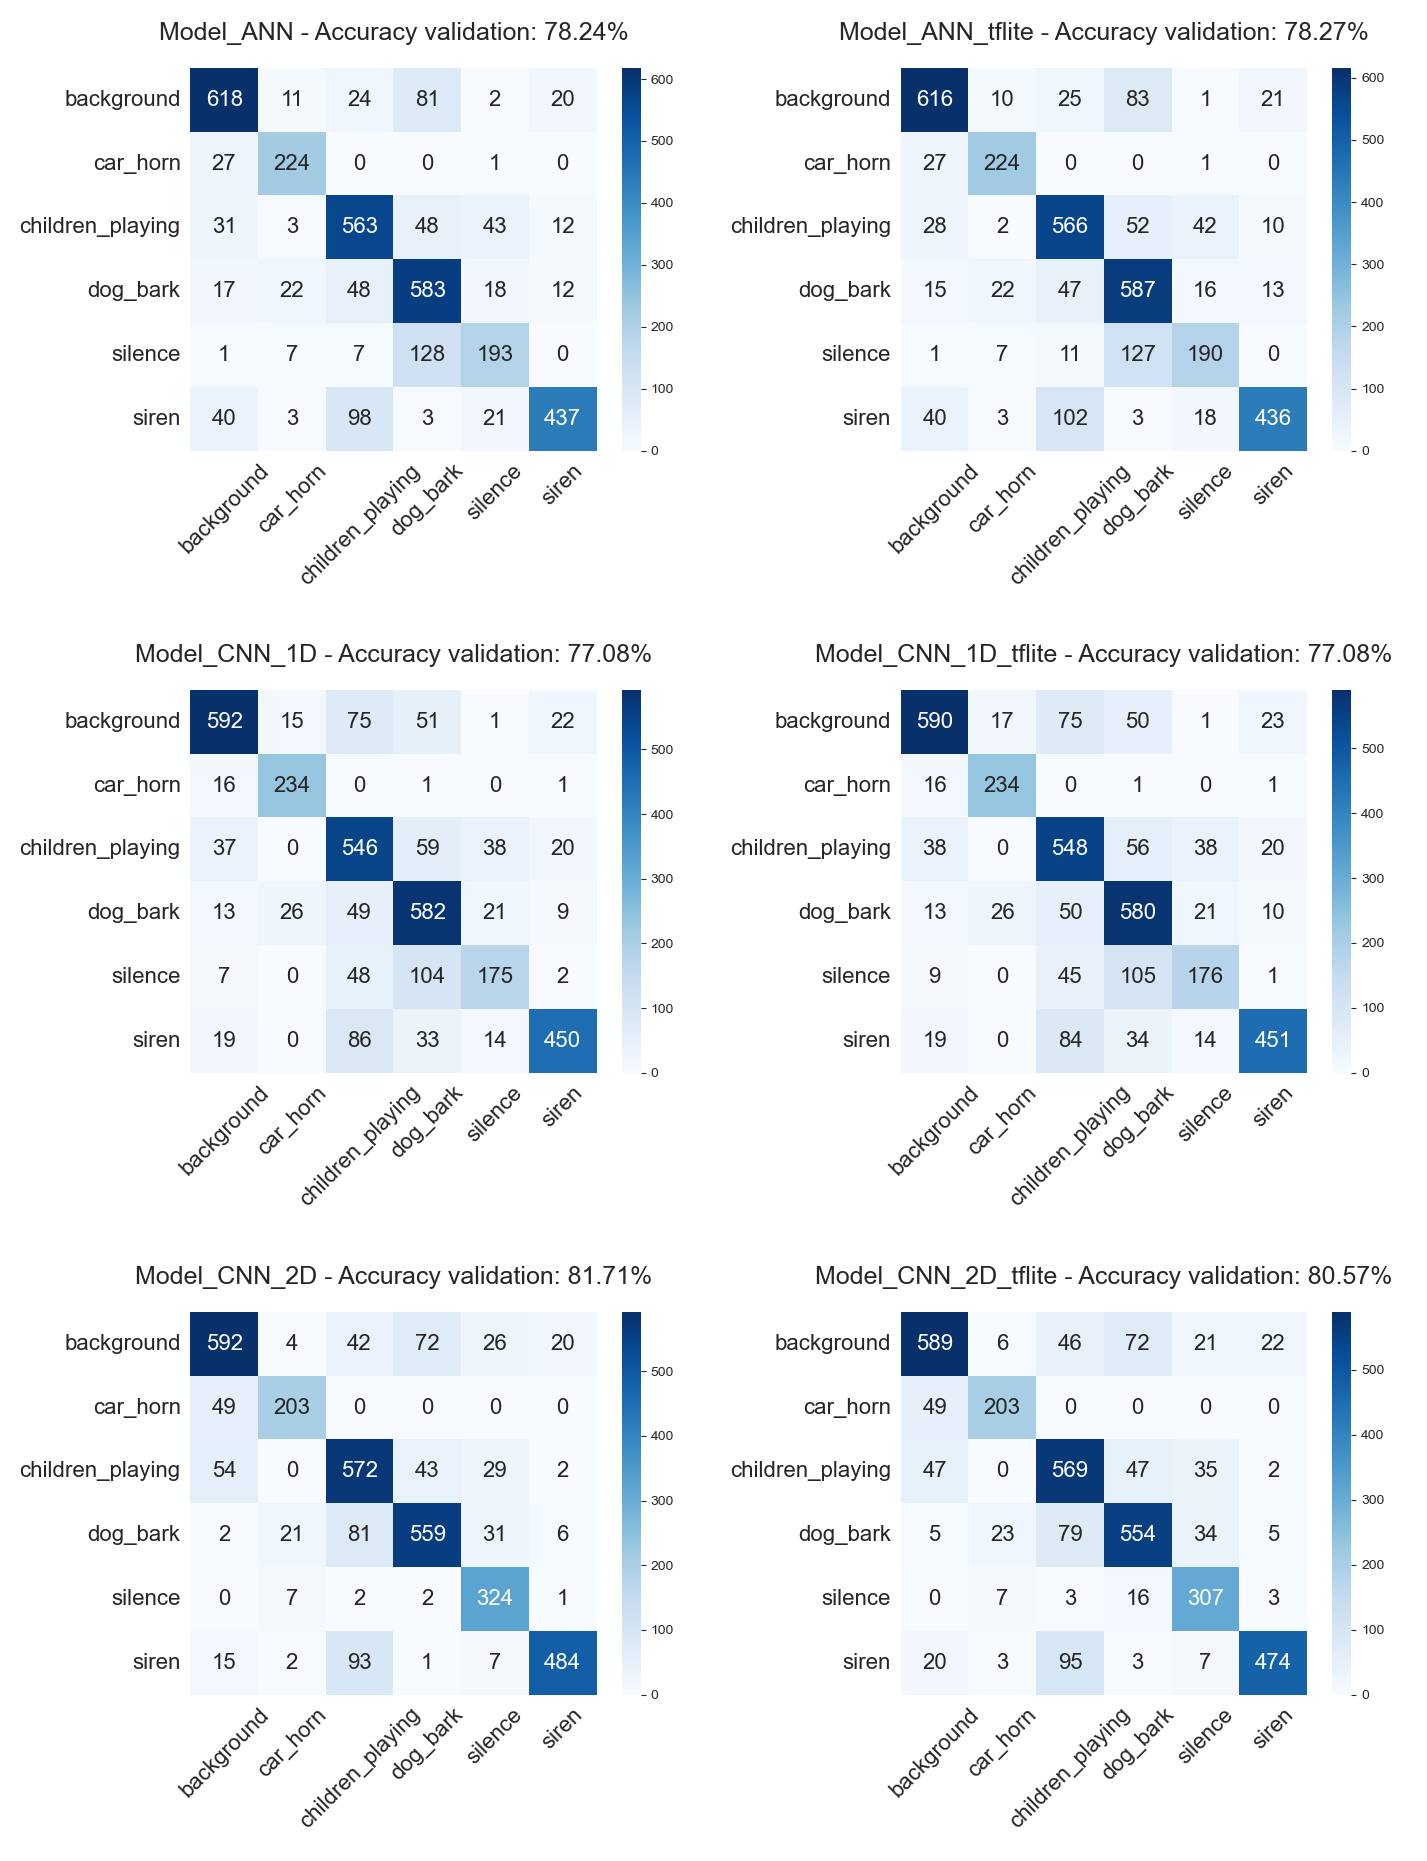
\includegraphics[width=1\textwidth]{resources/images/060-results/Results_classification_overview_models_evaluation_2.png}
        \smallcaption{Source: Author}
        \label{fig:Results_nn_models_evaluation}
\end{figure}

To compare an algorithm's performance in a notebook and a Raspberry Pi, both devices must be in good condition with similar operating systems. The same algorithm version and development environment should be used to ensure equivalent workloads, monitor temperature to prevent throttling, and execute multiple tests to obtain a reliable average. Differences in processor architectures (x86 vs. ARM) and the algorithm's ability to utilize multiple cores should be considered. Evaluation of scheduling policies, memory management, and potential conflicts of shared resources among cores is also necessary. Given that the objective of this study is not a quantitative comparison \textit{per se} of these devices but rather a qualitative one, all these factors were verified superficially. The averaged results of the comparison between the top-performing predictive models after 10 loops were compiled in Table \ref{table:results_classifiers_performance_us8k_av}, reporting the total prediction time and the processing memory in both notebook and Raspberry Pi.

\begin{table}[ht!]
    \caption[Processing memory (RAM) and total prediction time.]{Processing memory (RAM) and total prediction time. Comparison between the predictive algorithms in the notebook and Raspberry Pi.}
    \label{table:results_classifiers_performance_us8k_av}
    \centering
    \begin{tabular}{
        >{\raggedright\arraybackslash}m{0.16\textwidth} | >
        {\raggedright\arraybackslash}m{0.15\textwidth} | >
        {\raggedright\arraybackslash}m{0.19\textwidth} | >
        {\raggedright\arraybackslash}m{0.15\textwidth} | >       
        {\raggedright\arraybackslash}m{0.20\textwidth}}
        \Xhline{2\arrayrulewidth}
        \rowcolor{lightgray}
        \textbf{Classifier} & \centering\textbf{Notebook} & \centering\textbf{Notebook} & \centering\textbf{Raspberry Pi} & \centering\textbf{Raspberry Pi} \cr
        \rowcolor{lightgray}
         & \gls{ram} \hfill (Std) & Pred. time \hfill (Std) & \gls{ram} \hfill (Std) & Pred. time \hfill (Std) \cr
        \rowcolor{lightgray}
        & \centering (MB) & \centering (ms) & \centering (MB) & \centering (ms) \cr
        \hline
        \gls{svm}    & 34.1  \hfill(4.7)  & 223.4 \hfill(11.4) &  32.4  \hfill(8.2)  & 764.4   \hfill(39.6)   \\
        \gls{lr}     & 1.1   \hfill(0.1)  & 220.7 \hfill(11.8) &  0.2   \hfill(0.03) & 749.2   \hfill(14.6)   \\
        \gls{rf}     & 401.1 \hfill(65.4) & 227.2 \hfill(12.9) &  456.0 \hfill(11.3) & 1,020.9 \hfill(31.1)   \\
        \gls{ann}    & 20.6  \hfill(9.2)  & 250.1 \hfill(16.0) &  0.1   \hfill(0.02) & 752.5   \hfill(12.5)   \\
        \gls{cnn} 1D & 7.5   \hfill(0.5)  & 252.1 \hfill(20.0) &  4.1   \hfill(1.9)  & 750.0   \hfill(13.6)   \\
        \gls{cnn} 2D & 11.7  \hfill(0.2)  & 30.2  \hfill(7.2)  &  19.4  \hfill(2.5)  & 47.6    \hfill(22.0)   \\
    \Xhline{2\arrayrulewidth}
    \end{tabular}
    \smallcaption{Source: Author}
\end{table}

Additionally, the non-volatile storage medium that retains data even when the power is turned off (Flash memory) was also evaluated. In this study, the Flash memory represents the size of the predictive models, sorted by size as follows: 19.0 \gls{k}\gls{b} (\gls{lr}), 6,218.0 \gls{k}\gls{b} (\gls{cnn} 1D), 8,928.0 \gls{k}\gls{b} (\gls{ann}), 11,920.0 \gls{k}\gls{b} (\gls{cnn} 2D), 32,761.0 \gls{k}\gls{b} (\gls{svm}) and 249,522.0 \gls{k}\gls{b} (\gls{rf}). This information was normalized (min -1\% and max +1\% to avoid zero in the log axis) with the values of RAM and total prediction time to create the spider web chart depicted in Figure \ref{fig:Results_spider_chart_us8k_av_cnn2d}, which supports the decision of the predictive algorithm with \textbf{\gls{cnn} 2D} embedded in the Raspberry Pi.

\begin{figure}[htbp]
    \raggedright
        \caption{Spider web chart of the predictive algorithms.}
        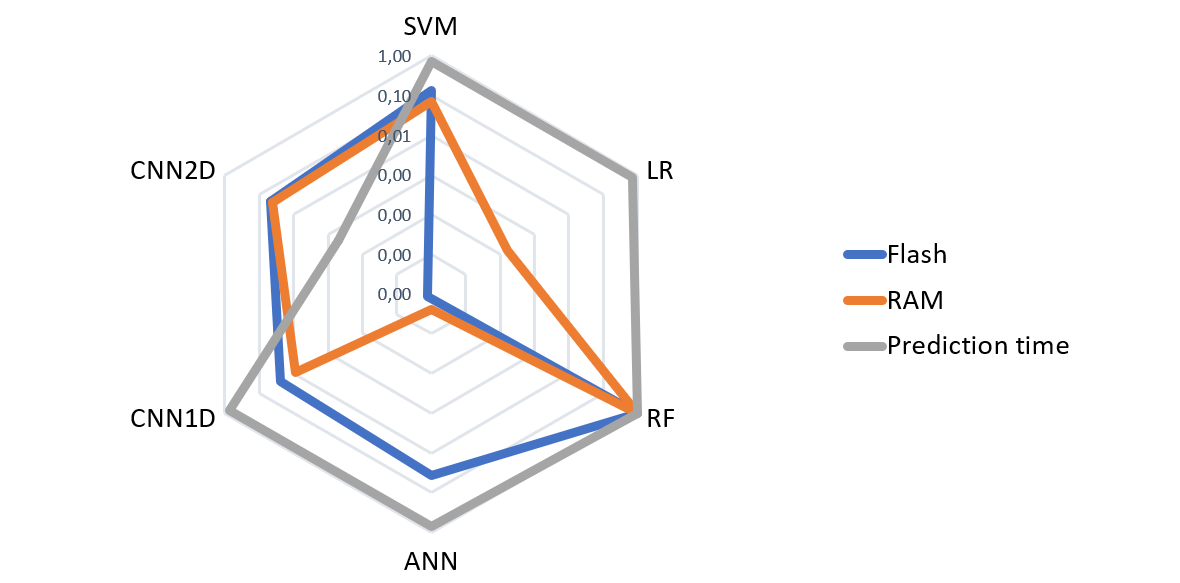
\includegraphics[width=1\textwidth]{resources/images/060-results/Results_spider_chart_us8k_av_cnn2d.png}
        \smallcaption{Source: Author}
        \label{fig:Results_spider_chart_us8k_av_cnn2d}
\end{figure}

Prior to the evaluation flow, an indoor experiment, as described in section \ref{sec:methods_evaluation}, was conducted to assess the effectiveness of the predictive algorithm \gls{cnn} 2D. The experimental setup comprised a notebook, a Raspberry Pi, and identical microphones arranged in a meeting room with an average background noise level of 60 \gls{db}, primarily due to air conditioning. The sound source was positioned 5 meters away from the microphones and approximately 120 \gls{s} of audio from YouTube was played at maximum volume on an iPhone 11, resulting in the generation of 107 audio samples. The \gls{spl} measured at the microphones reached a peak of 75 \gls{db} during playback but predominantly ranged between 60 \gls{db} and 65 \gls{db} due to the blending with background noise. The result of this experiment is presented in Table \ref{table:results_indoor_experiments} and inferred a sound algorithm with high precision and weighted F1-score ranging from 77\% to 95\%, both per analyzed class. 

\begin{table}[ht!]
    \caption[Classification metrics of the indoor experiments.]{Classification metrics of the indoor experiments.}
    \label{table:results_indoor_experiments}
    \centering
    \begin{tabular}{
        >{\raggedright\arraybackslash}m{0.26\textwidth} | >
        {\centering\arraybackslash}m{0.15\textwidth} | >
        {\centering\arraybackslash}m{0.15\textwidth} | >
        {\centering\arraybackslash}m{0.15\textwidth} | >
        {\centering\arraybackslash}m{0.15\textwidth}}
        \Xhline{2\arrayrulewidth}
        \rowcolor{lightgray}
        \textbf{Classes} & \textbf{Precision} & \textbf{Recall} & \textbf{F1-score} & \textbf{Samples} \\
        \hline
        \rowcolor{gray!20}
        Played: \hfill dog\_bark & & & & \\
        background        & 60.0\%  & 86.0\%  & 71.0\%  & 14  \\
        children playing  & 0.0\%   & 0.0\%   & 0.0\%   & 0   \\
        dog\_bark         & 97.0\%  & 65.0\%  & 77.0\%  & 93  \\
        \hline
        Weighted avg      & 92.0\%  & 67.0\%  & 77.0\%  & 107 \\
        \hline
        \rowcolor{gray!20}
        Played: \hfill children\_playing & & & & \\
        background        & 0.0\%    & 0.0\%   & 0.0\%   & 0   \\
        car\_horn         & 0.0\%    & 0.0\%   & 0.0\%   & 0   \\
        children playing  & 100.0\%  & 86.0\%  & 92.0\%  & 107 \\
        \hline
        Weighted avg      & 100.0\%  & 86.0\%  & 92.0\%  & 107 \\
        \hline
        \rowcolor{gray!20}
        Played: \hfill car\_horn & & & & \\
        background        & 44.0\%   & 100.0\%  & 61.0\%  & 7   \\
        car\_horn         & 100.0\%  & 84.0\%   & 91.0\%  & 100 \\
        children playing  & 0.0\%    & 0.0\%    & 0.0\%   & 0   \\
        siren             & 0.0\%    & 0.0\%    & 0.0\%   & 0   \\
        \hline
        Weighted avg      & 96.0\%   & 85.0\%   & 89.0\%  & 107 \\
        \hline
        \rowcolor{gray!20}
        Played: \hfill siren & & & & \\
        background        & 67.0\%   & 100.0\%  & 80.0\%  & 2    \\
        children playing  & 0.0\%    & 0.0\%    & 0.0\%   & 0    \\
        dog\_bark         & 0.0\%    & 0.0\%    & 0.0\%   & 0    \\
        siren             & 100.0\%  & 90.0\%   & 95.0\%  & 105  \\
        \hline
        Weighted avg      & 99.0\%   & 91.0\%   & 95.0\%  & 107  \\
        \hline
     \Xhline{2\arrayrulewidth}
    \end{tabular}
    \smallcaption{Source: Author}
\end{table}


\section{EVALUATION FLOW}
\label{sec:results_evaluation_flow}

The evaluation process was conducted on the streets of Santo André and São Bernardo do Campo, SP, Brazil, during regular traffic hours. All vehicle windows were closed, the infotainment system was turned off (no music), there was no additional passenger inside the vehicle (no speech), and the air conditioning was set to level 2, producing an \gls{spl} near the microphones of approximately 65 \gls{db}. Both microphones were attached to the passenger sun visor near the vehicle's Bluetooth microphone.

The first experiment, designated "Driving on streets 01", aimed to evaluate the performance of the \gls{esr} algorithm under real driving conditions, with speeds ranging from 10 to 50 km/h and maximum \gls{spl} of 80 \gls{db}. This setting involved a broad soundscape typically encountered in large cities. The experiment lasted 3,690 \gls{s} ($\approx$1 hour) and produced 3,310 audio clips, each lasting approximately 1.114578 \gls{s} instead of the intended 1 \gls{s}. This discrepancy was caused by the chunk size of 8,192 samples used in the Raspberry Pi to prevent overflow during audio recording. 

Although none of the relevant classes (dog\_bark, children\_playing, car\_horn, and siren) were present during the experiment, the results demonstrated a robust algorithm with an F1-score reaching 99\%, as illustrated by the confusion matrix in Figure \ref{fig:Results_evaluation_driving_streets_01}.

\begin{figure}[htbp]
    \raggedright
        \caption{Confusion matrix of the first experiment, "Driving on streets 01" without the presence of relevant classes.}
        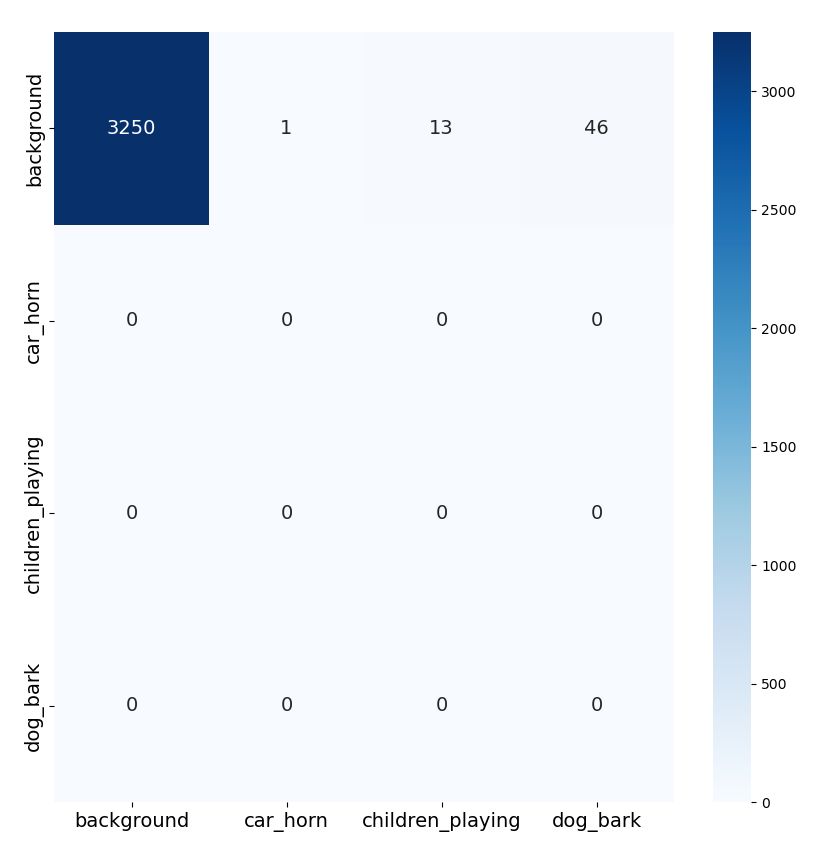
\includegraphics[width=.5\textwidth]{resources/images/060-results/Results_evaluation_driving_streets_01.png}
        \smallcaption{Source: Author}
        \label{fig:Results_evaluation_driving_streets_01}
\end{figure}

The chunk function in Python operates as a buffer, with each buffer containing 1,024 samples by default, which can then either be retained or discarded by the algorithm. If recorded and saved without segmentation, continuous data flow from a microphone would excessively consume processor resources and potentially lead to system crashes. To address this issue, most Python libraries utilize chunks of data instead of a continuous audio stream. While in the notebook, the chunk size can be set to lower values such as 256 or 512 without overflow problems, in the context of Raspberry Pi, where resources are limited, chunking the data with higher values (2,048, 4,096 or higher) facilitates smoother stream flow and prevents memory leaks. However, higher chunk sizes introduce some latency in the audio recording, on average a few dozen \gls{mi}\gls{s}, reaching no more than one hundred \gls{mi}\gls{s} at higher values.

In an effort to mitigate the latency induced by the chunk size of 8,192 samples employed in the \gls{esr} algorithm embedded in the Raspberry Pi, three experiments were conducted with the chunk size adjusted to 4,096, representing the upper limit before encountering buffer input overflow. For reference, the chunk size utilized in the notebook was set to 1,024 samples. 

The first experiment, titled "Driving on Streets 02", with one class of interest (siren), spanned a duration of 737 \gls{s} and resulted in the generation of 721 audio clips. The second experiment, "Driving on Streets 03", also with one class of interest (dog\_bark), had a considerably longer duration of 2,834 \gls{s} and produced 2,774 audio clips. The final experiment, "Driving on Streets 04", with two classes of interest (siren and car\_horn), lasted for 1,368 \gls{s} and yielded 1,339 audio clips. Each of these experiments produced audio clips with approximately 1.021678 \gls{s} instead of 1.114578 \gls{s}, nevertheless, the weighted F1-score in all three experiments was considerably lower, reaching 50\%, 22\% and 50\% respectively.

By comparing the audio clip recorded in the Raspberry Pi with the corresponding segment from the continuous audio recorded in the notebook, it is evident that the reduction in chunk size induced artifacts (distortions) across various frequency bands, as illustrated in Figure \ref{fig:Results_evaluation_driving_streets_02_04}, and adversely affected the inferences generated by the predictive algorithm. These distortions were also subjectively confirmed by manually listening and comparing the audio clips.

\begin{figure}[htbp]
    \raggedright
        \caption{Comparison between the audio clip recorded with chunk = 4,096 in the Raspberry Pi and the continuous audio recorded in the notebook.}
        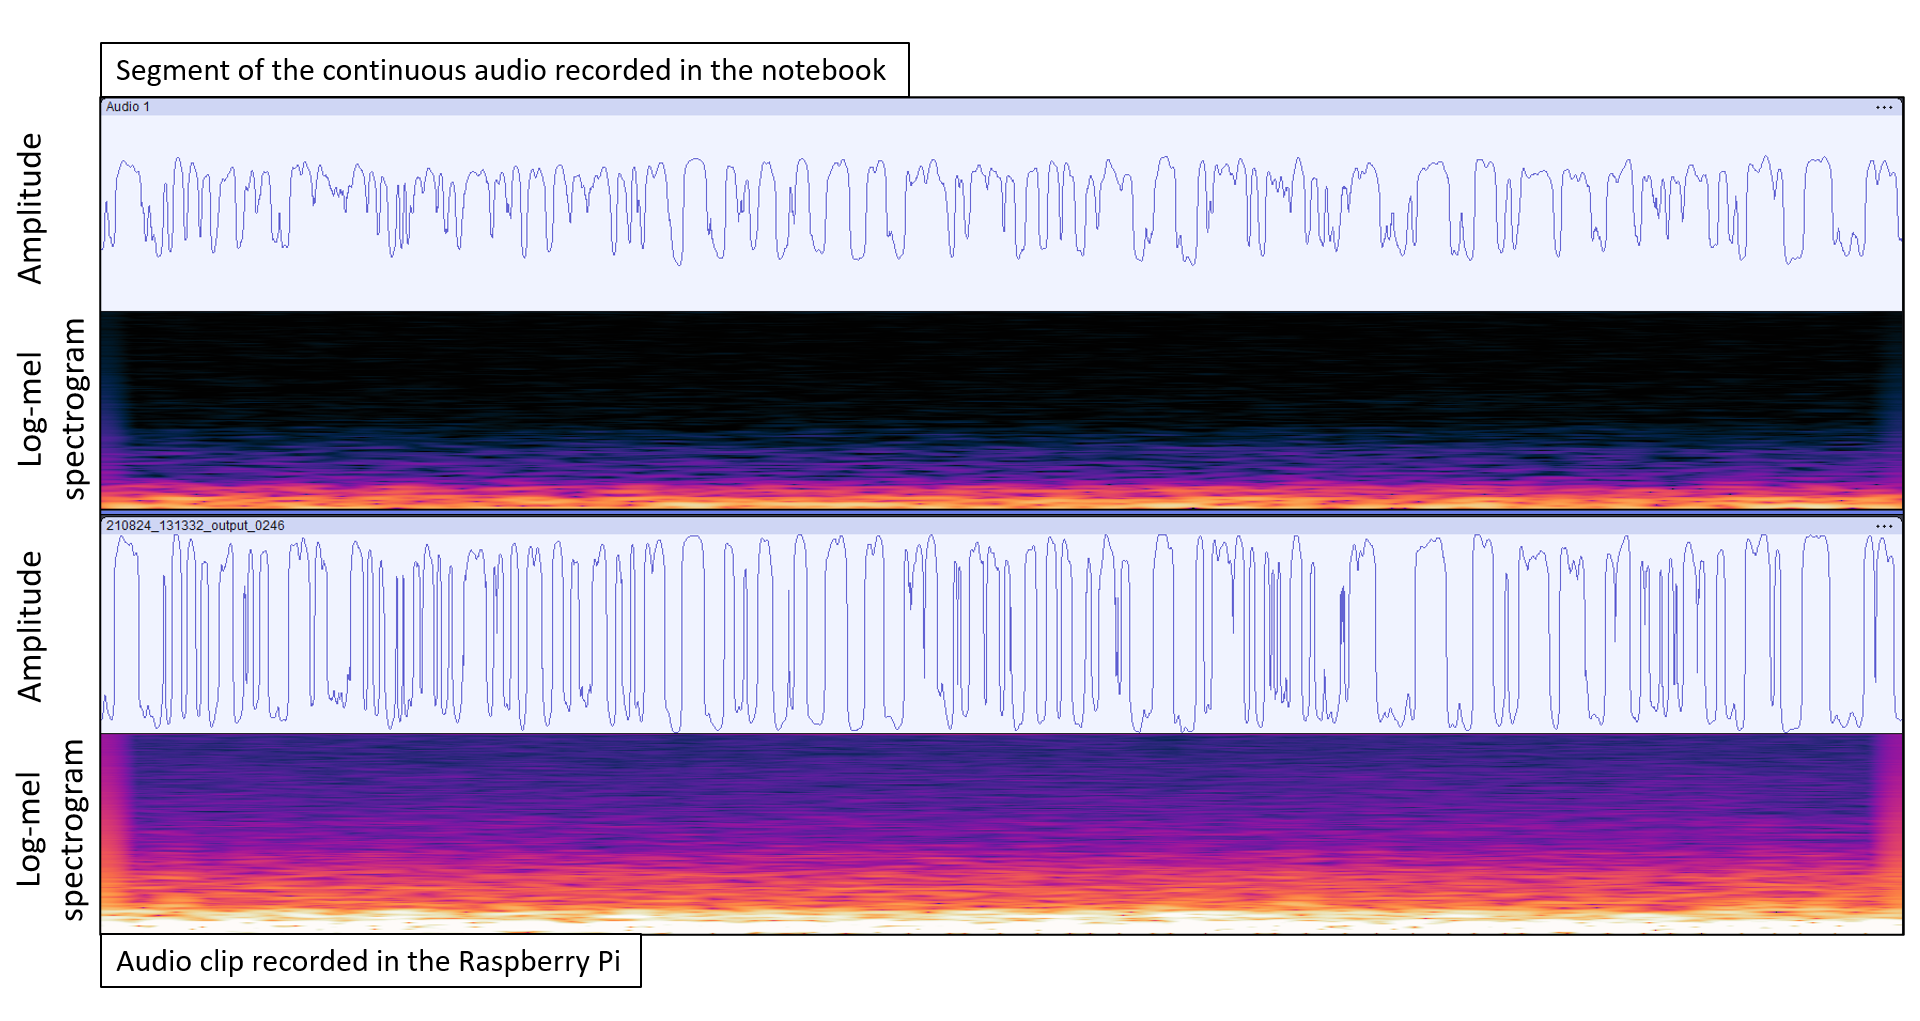
\includegraphics[width=1\textwidth]{resources/images/060-results/Results_evaluation_driving_streets_02_04.png}
        \smallcaption{Source: Author}
        \label{fig:Results_evaluation_driving_streets_02_04}
\end{figure}

Once the optimal chunk size for the Raspberry Pi was established at 8,192 samples, the objective of the subsequent experiments was to decisively identify four relevant sound classes: dog\_bark, children\_playing, car\_horn, and siren. A cumulative duration exceeding 10 hours of audio recordings was obtained through regular driving, as initially described in this section. However, as anticipated, the acquisition of sounds pertaining to the dog\_bark and children\_playing classes proved challenging in urban street environments. These sounds are predominantly encountered in leisure areas and parks, which are indeed target operational environments for the C-Bot. Consequently, the experiments for these two classes were conducted with the vehicle in a stationary position rather than in motion but maintained all other specifications previously described.

The experiment designated "Driving on streets 05" consisted of approximately 90 \gls{s} of recording with the sound-emitting source (a single dog) situated around 5 meters away in a pet park. This experiment produced 81 audio clips. The second stationary experiment, "Driving on streets 06", extended for 293 \gls{s}, yielding 263 audio clips, and involved approximately 15 children playing in "Cidade da Criança" park, located between 10 and 15 meters from the parked vehicle.

The experiment "Driving on streets 07" took place in a parking lot and lasted for 210 \gls{s}, producing 188 audio clips. This experiment aimed to evaluate the car\_horn class and included two phases: during the first half, the sound-emitting source was static (parked vehicle), while the vehicle equipped with the \gls{esr} algorithm was in motion at approximately 30 km/h. The parked vehicle started to honk its horn when the moving vehicle was around 30 meters away; it continued honking as it passed by at the closest distance of 4 meters and stopped when the distance reached around 30 meters again. During the second half of the experiment, both vehicles were in motion, maintaining an approximate distance of 10 meters from each other.

Finally, the last experiment, titled "Driving on streets 08", was conducted in a neighborhood characterized by numerous hospitals and trauma centers. This experiment had the longest duration with 2,425 \gls{s}. During this period, one event pertaining to the siren class was identified when an ambulance approached from the opposite direction to the vehicle equipped with the \gls{esr} algorithm. The ambulance was moving at a slow pace due to traffic congestion, while the vehicle equipped with the \gls{esr} algorithm maintained a speed of 25 km/h. The siren event lasted approximately 15 \gls{s}; notably, the ambulance was not visible to the driver at the beginning of the event for a few seconds during this period. Assuming the ambulance is stationary, the speed of the vehicle with the \gls{esr} algorithm, and the event duration, it is possible to infer that the ambulance was approximately 100 meters away when the event started.

The inference results from these four experiments have been compiled in Table \ref{table:results_outdoor_experiments}.

\begin{table}[ht!]
    \caption[Classification metrics of the outdoor experiments.]{Classification metrics of the outdoor experiments.}
    \label{table:results_outdoor_experiments}
    \centering
    \begin{tabular}{
        >{\raggedright\arraybackslash}m{0.26\textwidth} | >
        {\centering\arraybackslash}m{0.15\textwidth} | >
        {\centering\arraybackslash}m{0.15\textwidth} | >
        {\centering\arraybackslash}m{0.15\textwidth} | >
        {\centering\arraybackslash}m{0.15\textwidth}}
        \Xhline{2\arrayrulewidth}
        \rowcolor{lightgray}
        \textbf{Classes} & \textbf{Precision} & \textbf{Recall} & \textbf{F1-score} & \textbf{Samples} \\
        \hline
        \rowcolor{gray!20}
        Driving on the streets 05 & & & & \\
        background        & 94.0\%   & 85.0\%  & 89.0\%  & 40  \\
        children playing  & 0.0\%    & 0.0\%   & 0.0\%   & 0   \\
        dog\_bark         & 95.0\%   & 90.0\%  & 92.0\%  & 41  \\
        silence           & 0.0\%    & 0.0\%   & 0.0\%   & 0   \\
        \hline
        Weighted avg      & 95.0\%   & 88.0\%  & 91.0\%  & 81  \\
        \hline
        \rowcolor{gray!20}
        Driving on the streets 06 & & & & \\
        background        & 91.0\%    & 91.0\%  & 91.0\%  & 96   \\
        children playing  & 95.0\%    & 95.0\%  & 95.0\%  & 167  \\
        \hline
        Weighted avg      & 93.0\%    & 93.0\%  & 93.0\%  & 263  \\
        \hline
        \rowcolor{gray!20}
        Driving on the streets 07 & & & & \\
        background        & 98.0\%   & 94.0\%  & 96.0\%  & 171  \\
        car\_horn         & 100.0\%  & 59.0\%  & 74.0\%  & 17   \\
        children playing  & 0.0\%    & 0.0\%   & 0.0\%   & 0    \\
        dog\_bark         & 0.0\%    & 0.0\%   & 0.0\%   & 0    \\
        \hline
        Weighted avg      & 98.0\%    & 90.0\%  & 94.0\%  & 188  \\
        \hline
        \rowcolor{gray!20}
        Driving on the streets 08 & & & & \\
        background        & 100.0\%    & 99.0\%  & 99.0\%  & 2,163  \\
        children playing  & 0.0\%      & 0.0\%   & 0.0\%   & 0      \\
        dog\_bark         & 0.0\%      & 0.0\%   & 0.0\%   & 0      \\
        siren             & 65.0\%     & 85.0\%  & 73.0\%  & 13     \\
        \hline
        Weighted avg      & 100.0\%    & 99.0\%  & 99.0\%  & 2,176  \\
        \hline
     \Xhline{2\arrayrulewidth}
    \end{tabular}
    \smallcaption{Source: Author}
\end{table}

